

\documentclass[12pt]{article}
\usepackage[italian]{babel}
\usepackage[utf8x]{inputenc}
\usepackage{amsmath}
\usepackage{graphicx}
\usepackage[colorinlistoftodos]{todonotes}
\usepackage{algorithm2e}
\usepackage{algorithmic}
\usepackage{listings}
\usepackage{mathtools}
\DeclarePairedDelimiter{\ceil}{\lceil}{\rceil}
\usepackage{fancyhdr}
\usepackage[final]{pdfpages}


\pagestyle{fancy}
\fancyhf{}
\lhead{Relazione Progetto Laboratorio di Game Programming}


\begin{document}

\begin{titlepage}

\newcommand{\HRule}{\rule{\linewidth}{0.5mm}} % Defines a new command for the horizontal lines, change thickness here

\center % Center everything on the page
 
%----------------------------------------------------------------------------------------
%	HEADING SECTIONS
%----------------------------------------------------------------------------------------

\textsc{\LARGE Univeristà degli studi di Udine}\\[1.5cm] % Name of your university/college

%----------------------------------------------------------------------------------------
%	TITLE SECTION
%----------------------------------------------------------------------------------------

\HRule \\[0.4cm]
{ \huge \bfseries Progetto di Laboratorio di Game Programming}\\[0.4cm] % Title of your document
\HRule \\[1.5cm]
 
%----------------------------------------------------------------------------------------
%	AUTHOR SECTION
%----------------------------------------------------------------------------------------

\begin{minipage}{1\textwidth}
\begin{flushleft} \large
\emph{Autore:}\\
Fedrigo Mattia 138180 - fedrigo.mattia001@spes.uniud.it\\
Maestrutti Andrea 138461 - maestrutti.andrea@spes.uniud.it\\
Mauro Luca 138106 - mauro.luca001@spes.uniud.it\\
Not Simone 139032 - not.simone@spes.uniud.it\\

\end{flushleft}
\end{minipage}
~
\begin{minipage}{0.4\textwidth}

\end{minipage}\\[2cm]

% If you don't want a supervisor, uncomment the two lines below and remove the section above
%\Large \emph{Author:}\\
%John \textsc{Smith}\\[3cm] % Your name

%----------------------------------------------------------------------------------------
%	DATE SECTION
%----------------------------------------------------------------------------------------


%----------------------------------------------------------------------------------------
%	LOGO SECTION
%----------------------------------------------------------------------------------------


\includegraphics[width=50mm]{uniud.png}\\[1cm] % Include a department/university logo - this will require the graphicx package
 
%----------------------------------------------------------------------------------------

\vfill % Fill the rest of the page with whitespace

\end{titlepage}
\tableofcontents
\clearpage
\section{Il problema}
Il progetto d’esame relativo all’insegnamento di Laboratorio di Game Programming (LGP) consiste nell’implementazione di un videogioco utilizzando il framework di sviluppo CoronaSDK. Il tema del videogioco è l'ecologia e l'ambiente. 

Ai fini dello sviluppo è stato utilizzato il linguaggio di programmazione "Lua", che è un linguaggio utilizzato prevalentemente per scripting.


\textbf{NOTA}: Il codice, con i relativi moduli, è stato scritto interamente da noi. Si assicura che nulla è stato copiato o scaricato da progetti già esistenti. Buona parte degli assets sono stati realizzati utilizzando il software "Adobe Illustrator".
\subsection{Considerazioni}
La costruzione di un gioco su tematiche serie e istruttive quali l'ecologia e l'ambiente, non è mai un compito facile, specie per quanto concerne le componenenti di coinvolgimento e giocabilità che, parlando di un videogioco, devono essere tra gli aspetti principali. E' stato quindi deciso di creare un format ispirato ai classici del gioco mobile, con comandi semplificati al massimo e gameplay ispirati a successi internazionali: come "Jetpack Joyride" (per il movimento) e "Geometry Dash" (per l'atmosfera di gioco e grande precisione nei controlli richiesta nelle fasi avanzate del gioco). Abbiamo lavorato su questi elementi base, a cui abbiamo aggiunto le tematiche ambientali in modo coerente, stilizzando l'aspetto dei rifiuti e inserendo una meccanica abbastanza distintiva nel panorama dei runner infiniti, una barra della vita del mare, che si abbassa quando gli oggetti non vengono raccolti.

\section{Scopo del gioco}
Il gioco realizzato è intitolato \textbf{Save The Ocean}, il cui obiettivo è di liberare il fondale marino dalla spazzatura lasciata dall'uomo a bordo di un sommergibile, preservano così il pianeta e le creature dell'oceano.

La spazzatura è rappresentata da bottigliette di plastica e barili pieni di petrolio.


La sconfitta si verifica in due casi distinti: ogni qualvolta non si raccolga l'immondizia, oppure nel momento in cui il sommergibile vada a sbattere contro uno scoglio. Nel primo caso, non raccogliendo gli oggetti la "vita del mare" diminuisce e quando quest'ultima raggiunge la fine la partita finisce (raccogliendo gli oggetti, però, la vita del mare può essere recuperata); nel secondo caso, la partita termina immediatamente. 

L'utente dovrà raccogliere tutti i rifiuti presenti sul fondale marino. Ad ognuno corrisponde un punteggio differente: con la raccolta delle bottigliette di plastica si guadagnano 50 punti; mentre con la raccolta dei barili 150 punti.

Il gioco, inoltre, tiene traccia del punteggio massimo che viene raggiunto nelle varie sessioni.
Con il passare del tempo la velocità di gioco aumenta fino a raggiungere e mantenere la velcità massima, in particolare ogni 30 secondi viene aggiunto 0.25 al moltiplicatore dei punti. Con l'aumentare della velocità, aumenta anche la difficoltà quindi il giocatore dovrà essere il più abile possibile a raccogliere gli oggetti. 

Quando la partita termina compare la scritta \textbf{Game Over}, ed il giocatore può decidere se tornare al menù principale oppure ricominciare da capo la partita.
\section{Menù}
\subsection{What is it}
La schermata iniziale del gioco raffigura il menù, composto da tre pulsanti principali: il pulsante "play" che avvia la partita vera e propria; il pulsante "scores" che mostra i più alti punteggi ottenuti; ed infine il pulsante "about" che mostra le informazioni sugli sviluppatori ed il link al git se si volesse dare un proprio contributo al progetto. \\
\begin{center}
    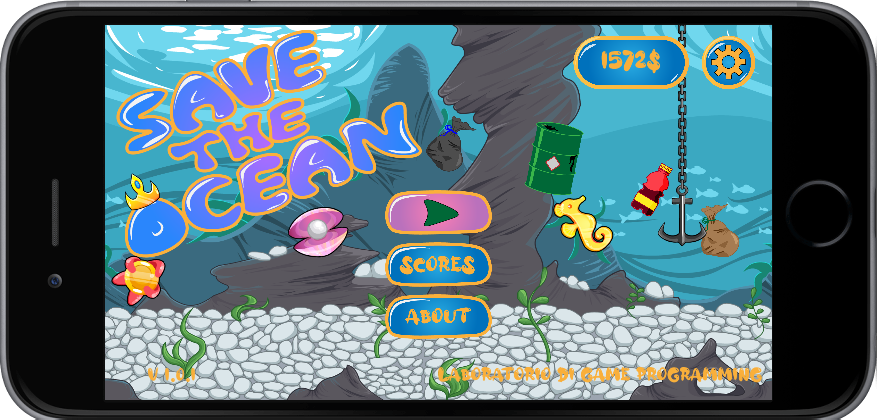
\includegraphics[width=80mm]{Menu.png}\\
\end{center}

Oltre ai 3 pulsanti principali, c'è anche un pulsante secondario raffigurato mediante un ingranaggio. Cliccandoci sopra si apre un menù a tendina che contiene altri 4 pulsanti:
\begin{itemize}
    \item uno realtivo alla scelta delle diverse skin del sottomarino; 
\begin{center}
    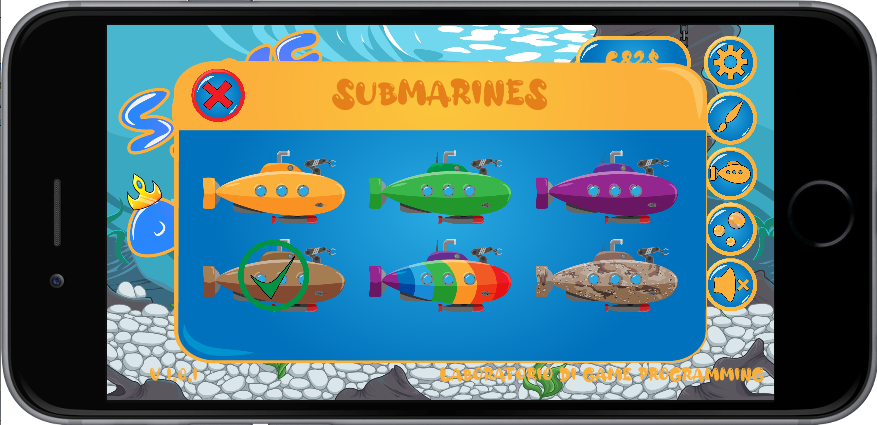
\includegraphics[width=80mm]{submarines.png}\\
\end{center}
    \item uno che mostra i vari ambienti di gioco selezionabili; 

\begin{center}
    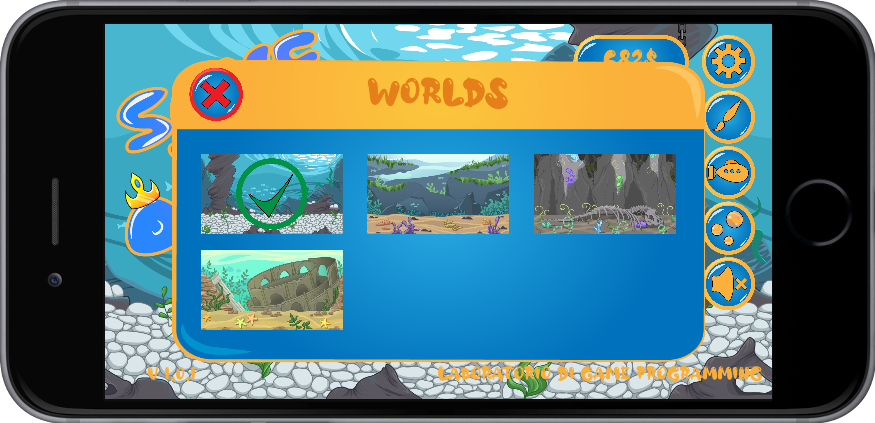
\includegraphics[width=80mm]{worlds.png}\\
\end{center}


    \item uno che permette la scelta del colore delle bolle che usciranno dal sottomarino. 
\\
\begin{center}
    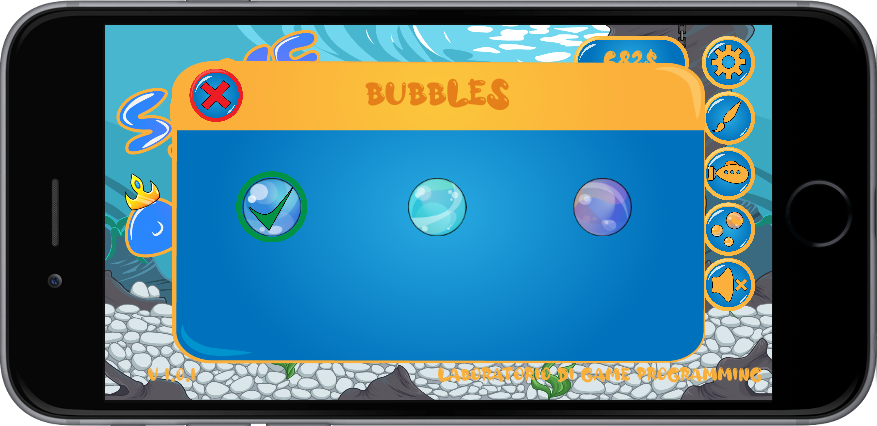
\includegraphics[width=80mm]{bubbles.png}\\
\end{center}

    \item infine uno che disabilita l'audio musicale. 
\end{itemize}

\subsection{Struttura}
\subsubsection{create()}
La funzione "create()" comincia la sua esecuzione impostando le variabili dei "displayObjects" degli oggetti da visualizzare (background e Ui). 

Nel create vengono inserite le immagini relative al titolo da visualizzare ed i vari pulsanti (play, scores, about...). Le immagini degli assets sono memorizzate all'interno di una cartella, e vengono caricate all'interno del gioco mediante la funzione "display.newImageRect" in cui viene indicato: il groupObject in cui inserire l'immagine; il file da cui caricare l'immagine; la directory di base in cui si trova filename; larghezza dell'immagine; altezza dell'immagine. 

I soldi posseduti dall'utente (che verranno poi utilizzati per acquistare skin del sottomarino, bolle oppure ambienti di gioco) sono indicati all'interno di un badge rettangolare avente gli angoli arrotondati. Anche in questo caso i vari asset sono stati caricati utilizzando la funzione "display.newImageRect". 

Nella parte bassa della scena del menù viene indicata la versione attuale del gioco e il titolo del corso. Entrambe sono state realizzate utilizzando la funzione "display.newText()", la quale crea un "text object". Dopo di che vengono impostati i valori degli attributi relativi all'altezza, alla larghezza, al colore e al posizionamento all'interno della scena. 

\textbf{NOTA:} come ausilio per il controllo del funzionamento degli acquisti, è possibile cliccare sopra il badge che contine la cifra dei soldi in possesso del giocatore per farli aumentare di 100\$ 

\subsubsection{show()}
Nel modulo relativo al menù, la funzione "show()" è stata implementata con lo scopo di riprodurre l'audio musicale su un canale, mediante la funzione "audio.play()".

\subsubsection{hide()}
La funzione "hide()", come detto in precedenza, è composta da due sottoeventi: nel "will" viene aggiornato il movimento del background mediante la funzione "timer.cancel()"; nel "did" viene stoppato tutto l'audio in esecuzione utilizzando "audio.stop()" (senza argomenti).

\subsubsection{destroy()}
Nel "destroy()" viene utilizzata la funzione "audio.dispose()" per stoppare l'audio relativo alla soundtrack del menù. 

\subsection{Librerie}
\subsubsection{About}
La liberia "About" non fa altro che mostrare a video una finestra in cui è contenuta un'immagine che rappresenta un testo relativo alle informazioni sugli sviluppatori e un link che reindirizza alla repository di github in cui è contenuto il codice. 

\subsubsection{Background}
La libreria "background" si occupa di gestire il movimento dello stesso all'interno della scena relativa al menù. Essendo la velocità impostata a 0.1, il background si muove in avanti e indietro molto lentamente, in modo tale da dare la sensazione di trovarsi effettivamente sott'acqua. A tal proposito viene usata la funzione "timer.performWithDelay()", che chiama una funzione specifica (BackgroundSpeedUpdate) dopo un intervallo di tempo stabilito. Tale funzione viene utilizzata per invertire il verso di scorrimento del background dopo un delay di 4 secondi. 
\subsubsection{Scores}
Lo score dipende da altri due moduli: "Window" e "Tabulator". Il suo compito è quello di mostrare delle targhette in cui sono contenuti i punteggi ottenuti dal giocatore. I primi tre punteggi sono inseriti all'interno di tre targhette "speciali" rispettivamente d'oro, d'argento e bronzo. Tutti gli altri punteggi invece all'interno di targhette normali. 
\subsubsection{Title}
La liberiea "Title.lua" si occupa di impostare il titolo (Save The Ocean) all'interno della scena e di inserire gli oggetti che fluttuano nel background. Il loro movimento deve essere gestito in modo particolare in quanto non possono non possono scontrarsi tra di loro. A questo proposito viene utilizzato un timer che va ad aggiornare le velocità di tali oggetti. Background e title sono stati separati perchè selezionando un nuovo world dalle impostazioni, aggiorna anche il background del menù e se fossero stati nella stessa libreria il ri-aggiornamento del background avrebbe sovrascritto sia il titolo del menù che gli oggetti che fluttuano.
\subsection{Settings}
Come detto in precedenza, all'interno del menù, oltre ai pulsanti principali, c'è un pulsante riguardante le impostazioni di gioco. L'oggetto selezionabile (skin, ambiente, bolla) viene rappresentato all'interno di una tabella in cui è indicato: il nome con cui è identificato; il percorso della cartella in cui è salvato; il prezzo da pagare per acquistarlo; una variabile booleana default, che indica se l'oggetto è aggiunto automaticamente agli oggetti dell'utente; ed una variabile booleana selected, che indica se l'oggetto è selezionato. 

Un oggetto non può essere selezionata se prima non è stato acquistato. A questo proposito si utilizza una funzione specifica in cui prima di tutto si verifica se è possibile acquistare l'oggetto in questione: se lo è, si seleziona quest'ultimo; se non lo è, mediante un file audio, si notifica all'utente che non ha abbastanza soldi. 
Ogni acquisto effettuato va a decrementare istantaneamente il denaro dalla scena principale.

Per gestire meglio questa parte di codice, si è deciso di creare 3 librerie differenti per i vari oggetti acquistabili.

\subsubsection{Bubbles}
La libreria "Bubbles" viene utilizzata per gestire la rappresentazione delle bolle e l'eventuale loro acquisto. Quest'ultime sono idientificate mediante un valore che va da 1 a 3. 
Per ognuna di esse vengono utilizzate due variabili necessarie al salvataggio: "submarineBubblesOwned", indica le bolle possedute dall'utente; "submarineBubblesSkin", indica la bolla selezionata dall'utente.
\subsubsection{Submarine}
La libreria "Submarines" permette di selezionare ed acquistare le skin dei sottomarini, che verranno poi utilizzate dall'utente durante il gioco. Nel caso sia il primo avvio del gioco, non ci saranno dati sui sottomarini posseduti e quindi verrà selezionato il sottomarino di default. 
Per ognuno di essi vengono utilizzate due variabili necessarie al salvataggio: "submarinesOwned", necessaria a memorizzare i sottomarini posseduti dall'utente; "submarineSkin", indica la skin del sottomarino selezionata dall'utente.
\subsubsection{Worlds}
Al fine di rendere il gioco più gradevole e meno monotono, sono stati inseriti vari ambienti di gioco differenti. 
Una volta che un background è stato acquistato e successivamente impostato, è necessario aggiornarlo non solo all'interno della partita ma anche all'interno della scena del menù mediante la funzione "updateBackground" inserita nella libreria "Background" citata in precedenza. 
Per ognuno di essi vengono utilizzate tre variabili, necessarie al salvataggio: "backgroundsOwned", necessaria a memorizzare gli ambienti di gioco posseduti dall'utente; "backgroundWorld", indica il tipo di ambiente selezionao dall'utente; ed infine, "backgroundLayerNum", il cui scopo è memorizzare il numero di layer di parallasse che compongono il background. 


\section{Game}
\subsection{What is it}
Dopo aver premuto il pulsante play si passa al file "game.lua", in cui vengono realizzati tutti gli oggetti ed il codice relativo 
alla realizzazione della logica del gioco.
\subsection{Struttura}
\subsubsection{create()}
Nella funzione create(), inzialmente vengono impostate le variabili legate al composer: "startTime", utilizzata per calcolare la 
velocità dello schermo in base al tempo; "gameSpeed", imposta la velocità iniziale di scorrimento dello schermo a 1. 
La velocità viene aggiornata ogni 1000 ms tramite un listener che chiama la funzione "updateGameSpeed". 
La scelta del valore 1000ms non è casuale, ma è stato inserito in modo tale da non accumulare troppo l'incremento in quel secondo.

Le collisioni tra sottomarino ed oggetti da raccogliere sono gestite a tempo di esecuzione mediante un listener, in questo modo ogni volta che avviene una collisione viene chiamata la funzione onCollision(). 

Il punteggio viene rappresentato mediante un "display object" in cui è stato utilizzato il font di default salvato in una variabile locale in modo tale da renderlo più accessibile in tutte le parti del programma. 

La vita del mare viene creata usando la funzione "newProgressView" in cui vengono inseriti 3 parametri:
\begin{itemize}
    \item percetuale della vita: rappresentata da un valore all'interno dell'intervallo [0,1] in cui 1 rappresenta il 100 e 0 lo 0. La barra viene creata inizialmente al 100.
    \item posizione della barra a seconda dell'asse X (inizialmente posta al centro dell'asse X)
    \item posizione della barra a seconda dell'asse Y
\end{itemize}

La percentuale di progresso della barra viene gestita da un metodo "setProgress" inserito all'interno della funzione newProgressView. Inoltre la vita del mare viene aggiornata utilizzando un timer: ogni secondo abbassa la vita del mare in funzione della quantità di oggetti che sono fuoriusciti dalla parte sinsitra schermo, e che quindi non sono stati raccolti dal sottomarino. 

\subsubsection{show()}
L'evento show() ha due sottoeventi chiamati "will" e "did". Nel "will" si aggiunge il timer che va ad aggiornare il moltiplicatore di punteggio: ogni 30 secondi si aggiunge 0.25 al moltiplicatore dei punti e la funzione che se ne occupa è "updateScoreMultiplier()". Il codice del sottoevento "did" viene eseguito non appena la scena è visualizzata sullo schermo, e come prima cosa viene riattivata la fisica, altrimenti il gioco inizierebbe con il sottomarino sulla parte bassa dello schermo. Inoltre, in questa fase, viene caricato il modulo relativo allo "spawner" dei vari oggetti(bottigliette, barili, scogli) e al caricamento dell'audio (la musica e i vari effetti sonori).

\subsubsection{hide()}
L'evento hide() viene usato per nascondere la scena, in particolare le sue funzioni vengono chiamate nella fase "did". Quando la scena è completamente off-screen, vengono eliminati i listener RunTime e i timer creati in precedenza. Una funzione particolarmente importante è "removeScene()" che rimuove completamente la scena, tutti gli oggetti e le variabili al suo interno,
in particolare si occupa degli oggetti all'interno della gerarchia di sceneGroup 
\\

\textbf{NOTA}: non rimuove costrutti come timer o listener collegati all'oggetto "Runtime". Essi vengono eliminati manualmente.

\subsubsection{destroy()}
L'evento destroy() viene utilizzato per eliminare l'audio prima della rimozione della scena.

\subsection{Funzioni}
In questo paragrafo verranno descritte le funzioni implementate per realizzare le funzionalità citate in precedenza.
\subsubsection{updateGameSpeed()}
La funzione che aggiorna la velocità di scorrimento dello schermo è chiamata "updateGameSpeed". Nella variabile "gs" viene memorizzata la velocità iniziale (inizializzata a 1). Tale valore viene confrontato periodicamente con la velocità massima raggiungibile (maxGameSpeed = 3) e, se strettamente minore, la variabile gs viene aggiornata in funzione del tempo trascorso mediante la formula:\\

\begin{center}
    gs = 1 + ( (os.time() - st) / 100 )
\end{center}

Dove \textbf{st} è lo "start time" e \textbf{os.time()} è una funzione che restituisce l'ora corrente in secondi a partire dal 1970.

\subsubsection{gameOver()}
La procedura "gameOver()", si occupa di gestire il caso in cui la partita termini: ovvero quando si va a sbattere contro uno scoglio oppure quando la vita del mare cala fino a raggiungere lo 0\%. Quando si verifica uno di questi due casi, la variabile "isGameOver" assume valore "true" e si interrompono tutti i suoni, la fisica del gioco, il movimento del background.\\

Il gameover è una scena che compare, mediante l'utilizzo del metodo degli overlay, sopra la scena principale, permettendo così al giocatore di scegliere se tornare al menù principale oppure ricominciare la partita.

Il modulo è impostato in modo tale che vengano disabilitate le pressioni sullo schermo relativo alla scena principale (quella di gioco). I dati da mostrare all'interno della finestra di gameover (lo score e i soldi guadagnati), vengono passati mediante una tabella dei parametri passata alla funzione "showOverlay()".

Quando si preme sul pulsante di riavvio della partita, si eliminano tutti gli elementi della scena precedente utilizzando (come suggerito dalla documentazione) una scena vuota chiamata dal  "refresh.lua", che contiene una funzione che rimanda ad una nuova scena del game.
\subsubsection{onCollision()}
Le collisioni sono gestite non in modo locale, bensì in globale dalla funzione “onCollision” aggiunta come
listener all’evento “collision” dell’oggetto Runtime.
La motivazione sta nel fatto che la tipologia di collisioni gestite è “molti a molti” e non
“uno a molti”. Infatti, per ridurre al minimo la quantità di oggetti raccoglibili ma non
prendibili, la collisione viene gestista anche nel caso in cui essi collidano con un
ostacolo (ovvero se l’ostacolo viene istanziato sopra all’oggetto raccoglibile), in questo
caso viene registrata la collisione e l’oggetto raccoglibile viene rimosso dal gioco senza
poi gravare sulla barra della vita del mare (e sull’estetica di gioco).

Per realizzare la procedura che gestisce la collisione tra gli oggetti è stato applicato il metodo dei filtri. 
Questo metodo implica l'assegnazione di \textbf{categoryBits} e \textbf{maskBits} agli oggetti tramite una definizione di una 
tabella assegnata al filtro durante la costruzione del corpo. Un oggetto entrerà in collisione con altri oggetti solo se i loro 
categoryBits sono tra i maskBits assegnati. Normalmente, un oggetto avrà solo un valore di categoryBits assegnato, ma potrebbe avere 
uno o più mskBits a seconda delle altre cose con cui dovrebbe entrare in collisione.

\begin{center}
    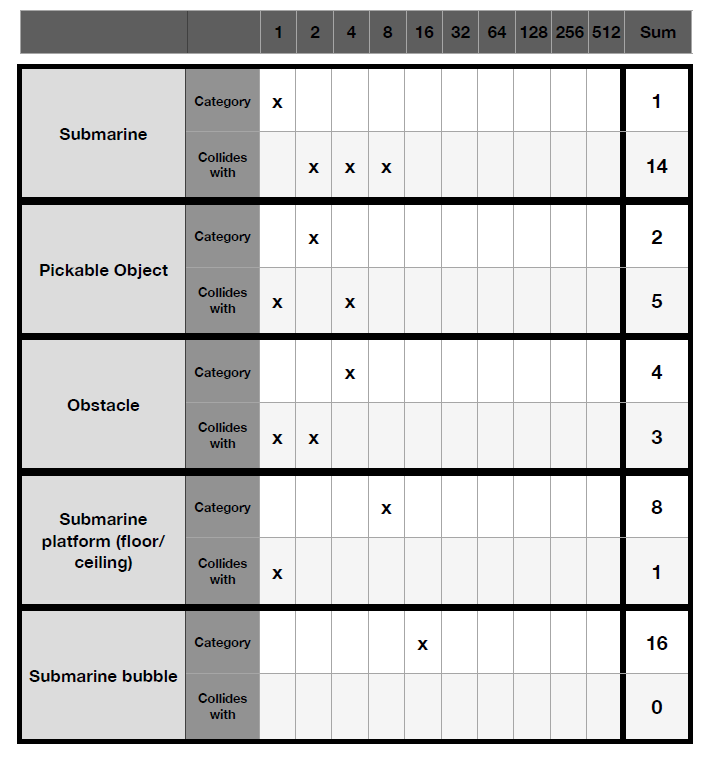
\includegraphics[width=110mm]{tabella2.png}\\
\end{center}

I parametri dei filtri sono stati impostati come "globali" sul composer, in quanto se in un secondo momento si aggiungono ulteriori 
elementi di gioco, è necessario lavorare di nuovo su tutti i tipi di oggetto: se il nuovo tipo di oggetto dovesse entrare in 
collisione con qualsiasi tipo di oggetto precedente, i valori di quest'ultimo potrebbero cambiare. 

\subsubsection{clearObject()}
Questa procedura si occupa di rimuovere tutti gli oggetti che escono dalla parte sinistra dello schermo (quindi quelli che non sono stati raccolti dall'utente) mediante le operazioni "display.remove(thisObject)" e "table.remove( screenObjectsTable, i)". "ScreenObjectTable" è una tabella in cui vengono inseriti tutti gli oggetti di gioco creati e quando si eliminano, vengono rimossi da essa. \\
Il ciclo for viene fatto partire dalla posizione finale della tabella, in quanto la funzione table.remove() è inefficiente (rimuovendo un oggetto dalla tabella, bisogna shiftare tutti gli oggetti in basso di una posizione in modo da mantenere la tabella compatta)

\subsubsection{updateSeaLife()}
Quando un oggetto non viene raccolto dall'utente la vita del mare cala del valore dell'oggetto perduto (ogni oggetto ha un valore differente). Questa funzione si occupa di aggiornare la vita quando si verifica la condizione appena citata ed utilizza la stessa tabella utilizzata nella funzione clearObject().
Per avere una risposta più rapida sulla barra della vita del mare in questo caso si va a contare la vita persa quando la coordinata "x" dell'oggetto diventa minore di 0.

Per ogni displayObject (quelli che si possono raccogliere) viene definito un attributo "mySeaLife", che viene utilizzato per evitare di contare più volte la vita del mare persa in base a questi oggetti (finchè l'oggetto, dopo essere uscito dallo schermo, non raggiunge -800, ogni volta che si va a richiamare il controllo per aggiornare la vita del mare si diminuisce la vita del valore di quell'oggetto). Quando il valore di seaLife è minore o uguale a 0, si richiama la funzione di gameOver().

Il controllo "isGameOver == false" viene effettuato altrimenti i suoni verrebbero riprodutti più volte.

\subsection{Librerie}
\subsubsection{background}
Lo scopo del modulo di background è quello di mostrare lo sfondo del gioco con un movimento che sfrutta l'effetto di parallasse. Inoltre, facendo scorrere ogni layer del background ad una velocità differente l'uno dall'altro, si ottiene un effetto di profondità.

Per gestire i diversi aspect ratio degli schermi presenti su smartphone sono state utilizzate tre immagini per ogni layer, poste una di fianco all'altra, di dimensioni 1920x1080p (aspect ratio 16:9). Questa strategia permette di coprire l'intera area di visione, utilizzando sempre la metodologia di scaling "letterbox", che non modifica l'aspet ratio delle immagini utilizzate (distorcendole), evitando allo stesso tempo le bande nere che deriverebbero dall'uso di questo tipo di scaling su smartphone con schermi più ampi nel senso della lunghezza.

\subsubsection{spawner}
Lo spawner è un modulo utilizzato per generare gli ostacoli e gli oggetti raccoglibili dal sottomarino, assegnano loro proprietà casuali di posizione, quantità, velocità e altri dettagli, molti dei quali dipendenti anche dalla velocità globale di gioco. A questo scopo è stata utilzzata la funzione "math.random", che viene utilizzata principalmente in tre circostanze: per generare il numero di oggetti che compariranno sullo schermo, per scegliere quali oggetti compariranno, per scegliere dove compariranno. Per la selezione dell’oggetto è stato possibile utilizzare i numeri in quanto ognuno di essi è identificato da un valore progressivo all'interno delle cartelle in cui è contenuto.

Dato che gli ostacoli devono avere una \textbf{hitbox} consistente con la loro forma, viene utillizzata la funzione di libreria 
graphics.newOutline(), per creare automaticamente il poligono della hitbox basandosi sulle sezioni col parmetro dell'ostacolo "alpha = 0" (trasparente).
Tale operazione richiede una certa elaborazione sull’immagine ed è onerosa in termini di prestazioni. E'stato dunque inserito un sistema 
dinamico di cache, che utilizza la table outlineCache dove vengono salvati gli output della funzione "graphics.newOutline()", utilizzando come stringa di riferimento per la tabella il nome del path dove risiede l’asset salvato (es. outlineCache [assetPathString] = graphics.newOutline() ).
Dunque ogni volta che è necessario creare l’outline di un ostacolo viene prima verificata la sua presenza all'interno della cache: se presente viene
estratto; se non presente viene generato, salvato nella cache, e poi letto.

Il sistema è dinamico, quindi non si basa 
su una tabella di nomi gia definita ma viene creata all’occorrenza e per qualsiasi nome di percorso.

\subsubsection{submarine}
Lo scopo del modulo "submarine.lua" è quello di gestire la generazione dell'oggetto submarine e la creazione delle bolle durante il suo movimento, oltre a tutti i parametri necessari per il funzionamento.
Il suo movimento è stato realizzato ispirandosi a quello del video-gioco "Jetpack Joyride", calibrandolo modificando la scala di gravità e la forza applicata verso l'alto ad esso quando si tiene premuto sullo schermo.\\

Per fare in modo che non esca dallo schermo sono stati utilizzati due quadrati statici: uno sul lato superiore ed uno sul lato inferiore dello schermo. Essendo dichiarati come statici essi hanno "massa infinita" e dunque non sono spostabili, vincolando di fatto il sottomarino nella posizione voluta.\\

È stato scelto di utilizzare una hitbox circolare per il sottomarino, invece di una più consistente outline dei bordi della figura per evitare problematiche col motore fisico box2D.
\\
L’unica parte inerente al movimento del sottomarino, non gestita tramite la fisica, è la rotazione: avviene durante il movimento, e viene gestita mediante la libreria "transition". La modifica di tale parametro (che in linea di massima è applicata molto spesso al sottomarino durante le interazioni), secondo quanto riportato nelle avvertenze, può causare crash nel motore grafico box2D, dal momento che la matematica alla base della collisione è ancora in fase di calcolo. Per ovviare a questo problema si è deciso dunque di utilizzare una semplice hitbox circolare attorno al sottomarino siccome, ruotando un cerchio attorno al suo centro la sua posizione e di conseguenza quella della sua area (la hitbox), rimane invariata, risolvendo alla radice possibili problematiche col movimento della hitbox durante l’elaborazione della collisione.

\section{Moduli globali}
In questo paragrafo verranno illustrate brevemente i principali moduli implementati, utilizzati per il corretto funzionamento del gioco:
\\
\subsection{Window}
Questa libreria si occupa della gestione di apertura e chiusura delle finestre con la relativa distruzione quando viene premuto il pulsante "x". Si occupa inoltre di formattare il testo nella posizione corretta all'interno dello schermo.
\subsection{Ui}
Libreria utilizzata per il posizionamento dei pulsanti e adesivi all'interno dell'interfaccia. Ha 3 modalità:
            \begin{itemize}
                \item posizionamento statico 
                \item unire i pulsanti sotto un pulsante "master" che si occupa di compattare e scompattare il menù di gioco
                \item apertura e chiusura con sostituzione del pulsante master
            \end{itemize}
\subsection{Tabulator} 
Si occupa di posizionare, come se si stesse creando una tabella, un determinato set di elementi, necessario per mostrare i vari elementi selezionabili come skin e highscores. Tramite una callback, che prende come parametro l'oggetto che è stato toccato, è possibile eseguire alcune operazioni su di esso, come per esempio selezionarlo o acquistarlo. Questa libreria offre due funzionalità legate all'oggetto di riferimento:
        \begin{itemize}
            \item stampare un badge sull’ oggetto
            \item stampare un altro oggetto sull'oggetto stesso
        \end{itemize}
\subsection{Audio} 
Esegue azioni sull'audio globale del gioco. Viene invocata nel main per caricare le impostazioni audio dal salvataggio al caricamento del gioco.
\subsection{Savedata}
Un modulo che ricopre una particolare importanza è senza dubbio il "savedata.lua", il quale si occupa di tenere in memoria i punteggi ottenuti dal giocatore, i soldi guadagnati, l'ultimo sottomarino utilizzato e l'ultimo ambiente in cui si ha effettuato la partita. Ogni dato di salvataggio è memorizzato in un file json, in particolare "gamedata.json" e "scores.json". 
Tutte le impostazioni di gioco  (skin, bolle, ambienti, punti, soldi) vengono conservate al'interno di "gamedata.json", che viene aperto in sola lettura mentre all'interno di "scores.json" vengono salvati i punteggi più alti. 

\section{Difficoltà riscontrate}
Per quanto riguarda le difficoltà riscontrate una delle principali riguarda la mancanza di documentazione adeguata relativa alle caratteristiche del linguaggio lua (es.scoping) e la scarsità di problematiche già risolte su siti appositi come StackOverflow. 
Dal lato implementativo, le uniche difficoltà sono state nella ricerca di eventuali errori, dovute all'assenza di strumenti di debugging.

\section{Pubblicazione}
Al fine di completare il ciclo di sviluppo dell'app, è stato deciso di proseguire fino in fondo, pubblicandola sul PlayStore.
L'app è stata pubblicata seguendo determinati passi:
\begin{itemize}
    \item per prima cosa è stata disegnata e creata l'icona che sarà il simbolo rappresentativo dell'app
    \item successivamente è stata generata una chiave di produzione in modo tale da poter firmare ufficialmente l'applicazione. Essa è necessaria alla pubblicazione.
    \item infine è stato avviato il beta test
\end{itemize}

L'applicazione è ancora in fase di approvazione.

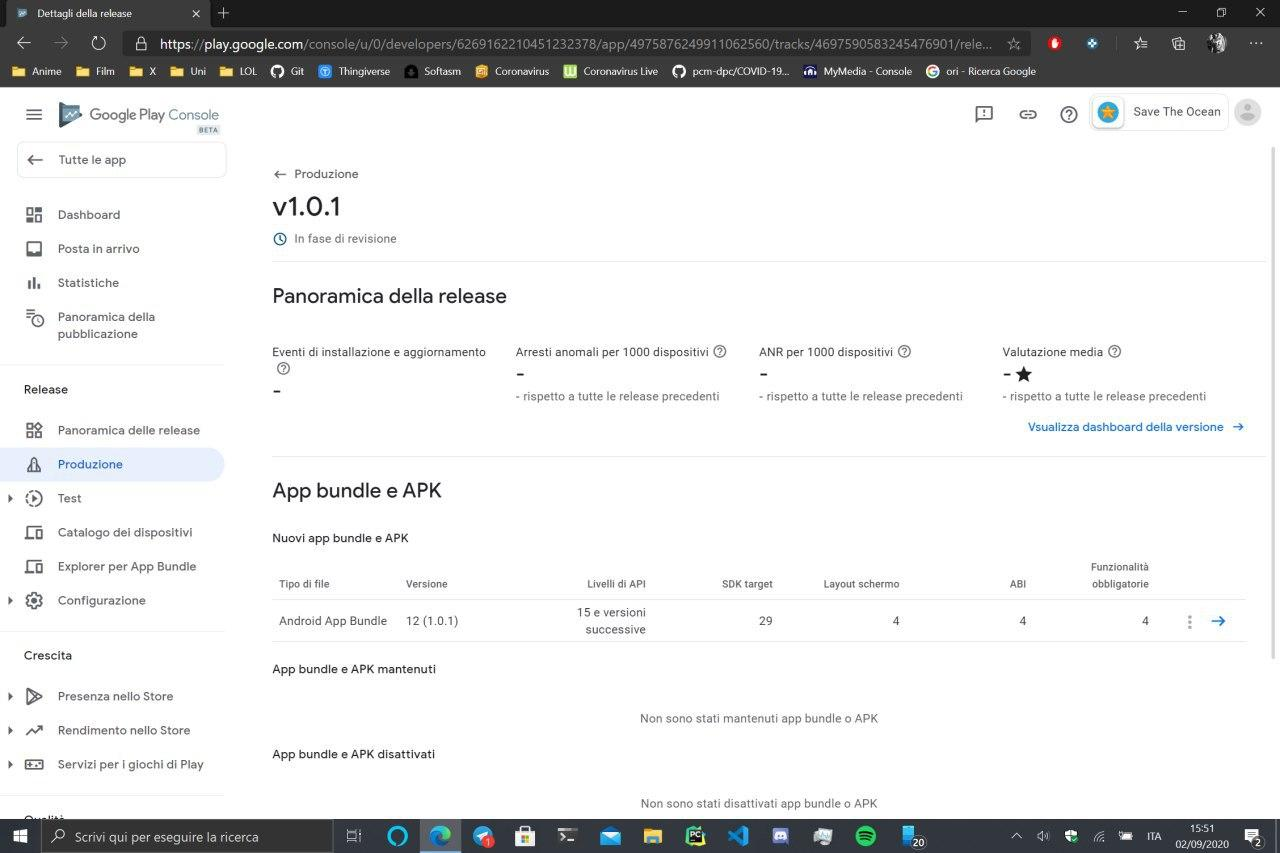
\includegraphics[width=110mm]{screen.jpg}
\end{document}